% Copyright (C) 2014-2020 by Thomas Auzinger <thomas@auzinger.name>

\documentclass[draft,final]{vutinfth} % Remove option 'final' to obtain debug information.

% Load packages to allow in- and output of non-ASCII characters.
\usepackage{lmodern}        % Use an extension of the original Computer Modern font to minimize the use of bitmapped letters.
\usepackage[T1]{fontenc}    % Determines font encoding of the output. Font packages have to be included before this line.
\usepackage[utf8]{inputenc} % Determines encoding of the input. All input files have to use UTF8 encoding.

% Extended LaTeX functionality is enables by including packages with \usepackage{...}.
\usepackage{amsmath}    % Extended typesetting of mathematical expression.
\usepackage{amssymb}    % Provides a multitude of mathematical symbols.
\usepackage{mathtools}  % Further extensions of mathematical typesetting.
\usepackage{microtype}  % Small-scale typographic enhancements.
\usepackage[inline]{enumitem} % User control over the layout of lists (itemize, enumerate, description).
\usepackage{multirow}   % Allows table elements to span several rows.
\usepackage{booktabs}   % Improves the typesettings of tables.
\usepackage{listings}   % Improves the typesettings of tables.
\usepackage{subcaption} % Allows the use of subfigures and enables their referencing.
\usepackage[ruled,linesnumbered,algochapter]{algorithm2e} % Enables the writing of pseudo code.
\usepackage[usenames,dvipsnames,table]{xcolor} % Allows the definition and use of colors. This package has to be included before tikz.
\usepackage{nag}       % Issues warnings when best practices in writing LaTeX documents are violated.
\usepackage{float} % Provides tooltip-like todo notes.
\usepackage{todonotes} % Provides tooltip-like todo notes.
\usepackage{hyperref}  % Enables cross linking in the electronic document version. This package has to be included second to last.
\usepackage{svg}
\usepackage[acronym,toc]{glossaries} % Enables the generation of glossaries and lists fo acronyms. This package has to be included last.

% Define convenience functions to use the author name and the thesis title in the PDF document properties.
\newcommand{\authorname}{Dragana Sunaric} % The author name without titles.
\newcommand{\thesistitle}{How to Model and Transform Executable BPMN Process Models} % The title of the thesis. The English version should be used, if it exists.

% Set PDF document properties
\hypersetup{
    pdfpagelayout   = TwoPageRight,           % How the document is shown in PDF viewers (optional).
    linkbordercolor = {Melon},                % The color of the borders of boxes around crosslinks (optional).
    pdfauthor       = {\authorname},          % The author's name in the document properties (optional).
    pdftitle        = {\thesistitle},         % The document's title in the document properties (optional).
    pdfsubject      = {Subject},              % The document's subject in the document properties (optional).
    pdfkeywords     = {a, list, of, keywords} % The document's keywords in the document properties (optional).
}

\definecolor{maroon}{rgb}{0.5,0,0}
\definecolor{darkgreen}{rgb}{0,0.5,0}
\lstdefinelanguage{XML}
{
	basicstyle=\ttfamily,
	morestring=[s]{"}{"},
	morecomment=[s]{?}{?},
	morecomment=[s]{!--}{--},
	commentstyle=\color{darkgreen},
	moredelim=[s][\color{black}]{>}{<},
	moredelim=[s][\color{red}]{\ }{=},
	stringstyle=\color{blue},
	identifierstyle=\color{maroon}
}

\setpnumwidth{2.5em}        % Avoid overfull hboxes in the table of contents (see memoir manual).
\setsecnumdepth{subsection} % Enumerate subsections.

\nonzeroparskip             % Create space between paragraphs (optional).
\setlength{\parindent}{0pt} % Remove paragraph identation (optional).

\makeindex      % Use an optional index.
\makeglossaries % Use an optional glossary.
%\glstocfalse   % Remove the glossaries from the table of contents.

% Set persons with 4 arguments:
%  {title before name}{name}{title after name}{gender}
%  where both titles are optional (i.e. can be given as empty brackets {}).
\setauthor{}{\authorname}{}{female}
\setadvisor{Ao.Univ.Prof. Dipl.-Inf. Dr.-Ing.}{Jürgen Dorn}{}{male}

% For bachelor and master theses:
%\setfirstassistant{Pretitle}{Forename Surname}{Posttitle}{male}
%\setsecondassistant{Pretitle}{Forename Surname}{Posttitle}{male}
%\setthirdassistant{Pretitle}{Forename Surname}{Posttitle}{male}

% Required data.
\setregnumber{11814569}
\setdate{01}{01}{2022} % Set date with 3 arguments: {day}{month}{year}.
\settitle{\thesistitle}{Vereinfachung von BPMN-Diagrammen} % Sets English and German version of the title (both can be English or German). If your title contains commas, enclose it with additional curvy brackets (i.e., {{your title}}) or define it as a macro as done with \thesistitle.
%\setsubtitle{Optional Subtitle of the Thesis}{Optionaler Untertitel der Arbeit} % Sets English and German version of the subtitle (both can be English or German).

% Select the thesis type: bachelor / master / doctor / phd-school.
% Bachelor:
\setthesis{bachelor}
%
% Master:
%\setthesis{master}
%\setmasterdegree{dipl.} % dipl. / rer.nat. / rer.soc.oec. / master
%
% Doctor:
%\setthesis{doctor}
%\setdoctordegree{rer.soc.oec.}% rer.nat. / techn. / rer.soc.oec.
%
% Doctor at the PhD School
%\setthesis{phd-school} % Deactivate non-English title pages (see below)

% For bachelor and master:
\setcurriculum{Software \& Information Engineering}{Software \& Information Engineering} % Sets the English and German name of the curriculum.

% For dissertations at the PhD School:
\setfirstreviewerdata{Affiliation, Country}
\setsecondreviewerdata{Affiliation, Country}


\begin{document}

% adding glossarys 
\newacronym{bpm}{BPM}{Business Process Management}
\newacronym{bpmn}{BPMN}{Business Process Model and Notation}
\newacronym{bpms}{BPMS}{Business Process Management System \gls{bpms-engine}}
\newacronym{XML}{XML}{Extensible Markup Language \gls{xml}}
\newacronym{wfms}{WfMS}{Workflow Managment System}
\newacronym{DMAIC}{DMAIC}{\textbf{D}efine, \textbf{M}easure, \textbf{A}nalyze, \textbf{I}mprove, \textbf{C}ontrol \cite{selvi2014six}}
\newacronym{DMADV}{DMADV}{\textbf{D}efine, \textbf{M}easure, \textbf{A}nalyze, \textbf{D}esign, \textbf{V}erify \cite{selvi2014six}}


\newacronym{XSD}{XSD}{XML Schema Definition \gls{xsd}}
\newglossaryentry{bpmn-wokflow-management-system}
{
	name={(BPMN) Workflow Management System},
	description={A software for executing workflows specified as \gls{bpmn} models}
}

\newglossaryentry{cycle-time}
{
	name={cycle time},
	description={The time it takes for a process from the start of the first task until the end of the last task \cite{Six-sigma-terms}}
}

\newglossaryentry{camunda}
{
	name={Camunda BPM},
	description={An enterprize Workflow-Management System written in java \cite{camunda-description}}
}
\newglossaryentry{alfresco}
{
	name={Alfresco Process Services (BPM)},
	description={Alfresco Process Services (powered by Activiti) is an enterprise Business Process Management (BPM) solution targeted at business people and developers. \cite{alfresco-description}}
}


\newglossaryentry{bpms-engine}
{
	name={Business Process Management System},
	description={see \gls{bpmn-wokflow-management-system}}
}

\newglossaryentry{executable-bpmn}
{
	name={executable \gls{bpmn} model},
	description={A software for executing workflows specified as \gls{bpmn} models}
}

\newglossaryentry{process-variables}
{
	name={Process Variables},
	description={Process variables are managed by the BPMS engine to allow data exchange between process elements}
}

\newglossaryentry{happy-path}
{
	name={'happy-path'},
	description={The best-case scenario in a process}
}

\newglossaryentry{conceptual-bpmn}
{
	name={conceptual \gls{bpmn} model},
	description={A \gls{bpmn} model describing a business process that cannot be directly executed on a \gls{bpmn-engine}}
}

\newglossaryentry{business-oriented-bpmn}
{
	name={business-oriented process model},
	description={See \gls{conceptual-bpmn}}
}
\newglossaryentry{automated-task}
{
	name={Automated task},
	description={A task that can be automated in a \gls{bpmn-wokflow-management-system}}
}

\newglossaryentry{service-task}
{
	name={Service Task},
	description={``Task that uses some sort of service, which could be a Web service or an automated application``\cite[p.~158]{bpmnstandard} }
}
\newglossaryentry{send-task}
{
	name={Send Task},
	description={``designed to send a Message to an external Participant``[p.~159]\cite{bpmnstandard} }
}
\newglossaryentry{receive-task}
{
	name={Receive Task},
	description={``designed to wait for a Message to arrive from an external Participant``[p.~161]\cite{bpmnstandard} }
}
\newglossaryentry{businessrule-task}
{
	name={Business Rule Task},
	description={``provides a mechanism for the Process to provide input to a Business Rules Engine and to get the output of calculations that the Business Rules Engine might provide``[p.~163]\cite{bpmnstandard} }
}
\newglossaryentry{script-task}
{
	name={Script Task},
	description={``executed by a business process engine. The modeler or implementer defines a script in a language that the engine can interpret``[p.~164]\cite{bpmnstandard} }
}
\newglossaryentry{manual-task}
{
	name={Manual Task},
	description={``A Task that is expected to be performed without the aid of any business process execution engine``[p.~163]\cite{bpmnstandard} }
}
\newglossaryentry{user-task}
{
	name={User Task},
	description={``A typical “workflow” Task where a human performer performs the Task with the assistance of a software application``[p.~163]\cite{bpmnstandard} }
}
\newglossaryentry{data-store}
{
	name={Data Store},
	description={``A DataStore provides a mechanism for Activities to retrieve or update stored information that will persist beyond the
		scope of the Process``[p.~208]\cite{bpmnstandard} }
}

\newglossaryentry{data-object}
{
	name={Data Object},
	description={``Data Objects representing a Collection of Data``[p.~206]\cite{bpmnstandard} }
}
\newglossaryentry{xml}
{
	name={XML},
	description={Extensible Markup Language - Defined by W3C\cite{bray1997extensibl} }
}

\newglossaryentry{xsd}
{
	name={XSD},
	description={XML Schema Definition - Definition of the stucture of a XML File\cite{bray1997extensibl} }
}

\frontmatter % Switches to roman numbering.
% The structure of the thesis has to conform to the guidelines at
%  https://informatics.tuwien.ac.at/study-services

%\addtitlepage{naustrian} % German title page (not for dissertations at the PhD School).

\selectlanguage{english}
\addtitlepage{english} % English title page.

\AddStatementPage



\begin{acknowledgements*}
	\todo{Ihr Text hier.}
	Lorem ipsum dolor sit amet, consetetur sadipscing elitr, sed diam nonumy eirmod tempor invidunt ut labore et dolore magna aliquyam erat, sed diam voluptua. At vero eos et accusam et justo duo dolores et ea rebum. Stet clita kasd gubergren, no sea takimata sanctus est Lorem ipsum dolor sit amet. Lorem ipsum dolor sit amet, consetetur sadipscing elitr, sed diam nonumy eirmod tempor invidunt ut labore et dolore magna aliquyam erat, sed diam voluptua. At vero eos et accusam et justo duo dolores et ea rebum. Stet clita kasd gubergren, no sea takimata sanctus est Lorem ipsum dolor sit amet. Lorem ipsum dolor sit amet, consetetur sadipscing elitr, sed diam nonumy eirmod tempor invidunt ut labore et dolore magna aliquyam erat, sed diam voluptua. At vero eos et accusam et justo duo dolores et ea rebum. Stet clita kasd gubergren, no sea takimata sanctus est Lorem ipsum dolor sit amet.   
	
	Duis autem vel eum iriure dolor in hendrerit in vulputate velit esse molestie consequat, vel illum dolore eu feugiat nulla facilisis at vero eros et accumsan et iusto odio dignissim qui blandit praesent luptatum zzril delenit augue duis dolore te feugait nulla facilisi. Lorem ipsum dolor sit amet, consectetuer adipiscing elit, sed diam nonummy nibh euismod tincidunt ut laoreet dolore magna aliquam erat volutpat.   
	
	Ut wisi enim ad minim veniam, quis nostrud exerci tation ullamcorper suscipit lobortis nisl ut aliquip ex ea commodo consequat. Duis autem vel eum iriure dolor in hendrerit in vulputate velit esse molestie consequat, vel illum dolore eu feugiat nulla facilisis at vero eros et accumsan et iusto odio dignissim qui blandit praesent luptatum zzril delenit augue duis dolore te feugait nulla facilisi.   
	
	Nam liber tempor cum soluta nobis eleifend option congue nihil imperdiet doming id quod mazim placerat facer
\end{acknowledgements*} % A short introduction to LaTeX.

\begin{abstract}	
BPMN is a commonly used diagramming language to visualize business processes. Executable process models are an effective tool for bridging the gap between IT experts, that are responsible for process automation, and domain experts, who have insight knowledge about the process at hand. This thesis explains best practices for modeling and transforming executable BPMN process models to make these expressive and readable. 

Based on this best practices, a list of suggestions that can be used to improve an existing BPMN model was formulated. 

Since some best practices are candidates for automation, a software was implemented as part of this thesis that can scan a BPMN model for violations of mentioned best practices. This software is freely available as an open source project on github:  \url{https://github.com/dsunaric/epms-service}. 

This thesis goes then on to demonstrate in a case study how the software can be used as an aid to implement the suggestions. The process used for this case study originated from a real live client registration process used in the telecommunication sector and was adapted to be used in this thesis.
\end{abstract}

% Select the language of the thesis, e.g., english or naustrian.

% Add a table of contents (toc).
\tableofcontents % Starred version, i.e., \tableofcontents*, removes the self-entry.

% Switch to arabic numbering and start the enumeration of chapters in the table of content.
\mainmatter

\chapter{Introduction}

\todo{write Introduction}

%Every organization has established internal processes that have to be managed. In order to be able to analyse and optimize these processes they firstly need to be specified. The established standard for visualizing business processes graphically is \gls{bpmn}. \cite{fundamentals} 

%Furthermore a graphical \gls{bpmn} model can build a bridge between \gls{bpm} experts and software engineers when there should be a common understanding about how the process works. IT-specialists have an important role in \gls{bpm} since the goal should be, once the processes of an organization are defined, to automate them as much as possible using computers. \cite{praxishandbuch}

%The advantage of using \gls{bpmn} instead of other specification languages for business processes is that it can easily be automated using \gls{bpms}. These \gls{bpms} can directly execute a \cite{executable-bpmn}. A \gls{bpmn} model that is usually used by \gls{bpm} experts, is called a \gls{business-oriented-bpmn} and has to be transformed into an \gls{executable-bpmn} in order to be automated. \cite{fundamentals} 


%\section{Motivation}
%Automated processes in large organizations are usually more complex than the \hyperref{fig:comparison-executable-conceptual}{Pizza ordering process} and consist of many steps 
%A shorter (and therefore simpler) model is easier to understand by both party's.

%Another reason for reducing the number of tasks in a process is the overhead for creating and persisting a task by a BPMN engine. This might be negligent for automated steps in BPMN but the overhead starts becoming notable when having a lot of user-tasks (non-automated tasks) since there is also the overhead of assigning tasks to users and communication between users.

%Another practical issue with having many nodes in BPMN models is the enterprise pricing of BPMN Engines. Some BPMN engines have a pricing scheme according to process instances passing a node so reducing the number of nodes without taking away expressiveness might have an impact on the pricing model and licence needed. 


%\section{Goal}

%\section{Structure of this thesis}
%The following section will give a brief introduction about the structure of this thesis. 


%\section{Evaluation approach}

\chapter{Automating Business Processes}

The following chapter will provide an overview of the current research on executable \gls{bpmn} models. First it will discuss the motivation behind process automation and using \gls{wfms}s and the benefit it might bring to an organization. Then it will state the differences between an \gls{conceptual-bpmn}, that cannot be deployed on an \gls{wfms}, and an \gls{executable-bpmn}. Finally this chapter will list the steps necessary to turn an \gls{conceptual-bpmn} executable.

\section{Why automate Processes?}
Introducing an \gls{wfms} in an organization is often done in order to open the possibilities to automating parts of a process or even the whole process. While process automation is an perused goal, there are some quantifiable advantages to using a \gls{wfms} besides the possibility to automate certain process steps.
\begin{itemize}
	\item \textbf{Shorten process lifetimes}: Managing processes manually requires handling tasks such as starting sub-processes or handling handovers from one entity to another and can lead to unnecessary waiting periods between two tasks. By implementing an \gls{wfms} resource allocation and parallelization can be automated where possible to assure optimal use of process resources. \cite{gadatsch2020grundkurs}
	
	\item \textbf{Reduction in process cost}: By reducing process lifetimes and increase productivity due to better handling resources can reduce process costs \cite{gadatsch2020grundkurs} but due to the high price for \gls{bpmn-wokflow-management-system}s the overall cost does not have to decrease necessarily \cite{gruber2009profitability}.
	
	\item \textbf{Workload reduction}: As stated earlier, managing processes needs to be done either by an \gls{bpmn-wokflow-management-system} or manually which creates additional workload for an organization. Workloads for employees executing the processes are also kept steady due to dynamic resource assignment. \cite{fundamentals}\cite{gadatsch2020grundkurs}
	
	\item \textbf{Enforce rules}: Defining the processes that is then directly executed and controlled by an \gls{bpmn-wokflow-management-system} enables the organization to enforce the execution of the process at it is designed. Following Rules and Protocols can partially be automated and enforcing guidelines and laws in an organization becomes easier. \cite{fundamentals}
	
	\item \textbf{Create Transparency}: Using an \gls{bpmn-wokflow-management-system} provides insights to the actually processes that are executed in the organization. It makes it easier to determine the performance of the processes by providing historical information of completed process instances and provides insight of the current status of processes that are still in progress. \cite{gadatsch2020grundkurs}
\end{itemize}

\section{Executable vs Conceptual Process Models}
Process Models are inherently Business-oriented as their purpose is initially to define and visualize the processes happening in an organization. Business-oriented or  \gls{conceptual-bpmn} are meant to be read by domain experts and contain usually implicit information known to these domain experts \cite{fundamentals}. They are usually incomplete, meaning that not every possible outcome of a process is modeled. In fact, usually only the best-case scenario, also known as the \gls{happy-path}, of a process is modeled in an \gls{conceptual-bpmn} \cite{freund2019real}. \\~\\Because of this, business-oriented models cannot be executed in an \gls{bpmn-wokflow-management-system} as they are but have to be turned into an \gls{executable-bpmn}. \gls{executable-bpmn} are meant for IT-experts and should be a technical representation of the business process while still begin understandable by domain experts. They should leave no room for interpretation as they have to contain all the information necessary for the process to be executed using an \gls{bpmn-wokflow-management-system}. Besides the visual information, \gls{executable-bpmn} also need to contain execution properties like interface definitions and Variables that are used by the Process called \gls{process-variables}.\cite{fundamentals} \\~\\An algorithm on how to efficiently turn an \gls{conceptual-bpmn} executable as stated in the book \textit{Fundamentals of Business Process Management} \cite{fundamentals} is described in the next section. 

\section{Making Process Models executable}
As stated earlier, \gls{bpmn} models can not directly be executed by a \gls{bpms} but have to be converted from an \gls{conceptual-bpmn} into an \gls{executable-bpmn}. 

There are different approaches how an \gls{executable-bpmn} can be derived from a business-oriented \gls{conceptual-bpmn}. In \cite{fundamentals} performing such a transformation is broken down into 5 steps:
\begin{enumerate}
	\item Identify the automation boundaries
	\item Review manual tasks
	\item Complete the process model
	\item Bring the process model to an adequate granularity level
	\item Specify execution properties
\end{enumerate}

\subsection{Identify the automation boundaries}
The first step in turning an \gls{conceptual-bpmn} in an  \gls{executable-bpmn} is to identify which steps can be automated using a \gls{bpmn-wokflow-management-system}. 

Tasks which can inherently be automated are called \gls{automated-task}s \cite[p.~317]{fundamentals}. Taking a look at the BPMN 2.0 standard an \gls{automated-task} can be one of the following Task types:
\begin{itemize}
	\item \textbf{\gls{service-task}}: A Task that invokes a service. Can be a Webservice or a application code.
	\item \textbf{\gls{send-task}}: Used to send a message to an external participant (A participant that is not part of the process)
	\item \textbf{\gls{receive-task}}: Used to receive a message from an external participant
	\item \textbf{\gls{script-task}}: Executes a Script that can be interpreted by the \gls{bpmn-wokflow-management-system}
	\item \textbf{\gls{businessrule-task}}: Executes a rule. (e.g. provides input for a business rule engine and gets the output of that calculation)
\end{itemize}

\begin{figure}[h]
	\centering
	\begin{subfigure}[b]{0.18\columnwidth}
		\centering
		
\includegraphics[width=0.9\textwidth]{graphics/service-task}
		\subcaption{Service Task}
		\label{fig:servicetask}
	\end{subfigure}
	\begin{subfigure}[b]{0.18\columnwidth}
		\centering
		
\includegraphics[width=0.9\columnwidth]{graphics/send-task}
		\subcaption{Send Task}
		\label{fig:sendtask}
	\end{subfigure}
	\begin{subfigure}[b]{0.18\columnwidth}
		\centering
		
\includegraphics[width=0.9\columnwidth]{graphics/receive-task}
		\subcaption{Receive Task}
		\label{fig:receivetask}
	\end{subfigure}
	\begin{subfigure}[b]{0.18\columnwidth}
		\centering
		
\includegraphics[width=0.9\columnwidth]{graphics/script-task}
		\subcaption{Script Task}
		\label{fig:scripttask}
	\end{subfigure}
	\begin{subfigure}[b]{0.24\columnwidth}
		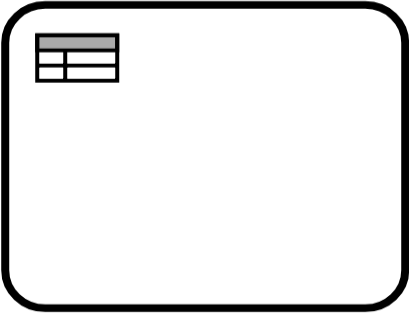
\includegraphics[width=0.675\columnwidth]{graphics/businessrule-task}
		\subcaption{Business Rule Task}
		\label{fig:businessruletask}
	\end{subfigure}
	\caption{Automated Tasks according to the BPMN 2.0 standard \cite{bpmnstandard}} % Remove the [...] argument if the original caption should be used in the figure list.
	\label{fig:automatedtasks} % \label has to be placed AFTER \caption (or \subcaption) to produce correct cross-references.
\end{figure}

Usually not every step of a Process can be fully automated. Processes can also have \textbf{\gls{manual-task}s} and \textbf{\gls{user-task}s}. A \textbf{\gls{user-task}} is a Task performed by a User with the aid of an \gls{bpmn-wokflow-management-system} while a \textbf{\gls{manual-task}} does not use any help from a business process execution engine. 

\begin{figure}[h]
	\centering
	\begin{subfigure}[b]{0.18\columnwidth}
		\centering
		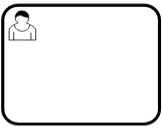
\includegraphics[width=0.9\textwidth]{graphics/user-task}
		\subcaption{User Task}
		\label{fig:usertask}
	\end{subfigure}
	\begin{subfigure}[b]{0.18\columnwidth}
		\centering
		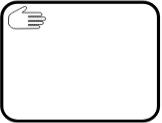
\includegraphics[width=0.9\columnwidth]{graphics/manual-task}
		\subcaption{Manual Task}
		\label{fig:manualtask}
	\end{subfigure}
	\caption{Manual and User Tasks according to the BPMN 2.0 standard \cite{bpmnstandard}} % Remove the [...] argument if the original caption should be used in the figure list.
	\label{fig:nonautomatedtasks} % \label has to be placed AFTER \caption (or \subcaption) to produce correct cross-references.
\end{figure}
\subsection{Review manual tasks}\label{manual}
As mentioned earlier \gls{manual-task}s are not automated and do also happen without the aid of a \gls{bpmn-wokflow-management-system}. In this step we need to analyse if the identified manual tasks in our \gls{bpmn}-model can be incorporated into the \gls{bpmn-wokflow-management-system}. This can be done in two ways:
\begin{itemize}
	\item \textbf{Automate the task}: Depending on the nature of the task that is currently performed manually, it might be possible to fully automate the task or to model the task as a \gls{receive-task} where the modelled task waits for a message that indicates the physical manual tasks completion.
	\item \textbf{Turn it into a User task}: If the task cannot be automated or the organization lacks the resources to automate the task yet, it might be possible to turn the \gls{manual-task} into a \gls{user-task}. One possibility could be to dedicate a person in charge of the manual task to notify the \gls{bpmn-wokflow-management-system} on the completion of the task via a worklist handler. \cite{stefanov2014business}
\end{itemize}

In the case that neither an \gls{automated-task} nor an \gls{user-task} is suitable for modelling the \gls{manual-task} one might also consider isolating the task and modelling the rest of the process. If this is also not possible due to the manual task being crucial for the expressiveness of the model it might be reconsidered if this process can or should be executed using a \gls{bpmn-wokflow-management-system}\cite[p.~228]{freund2019real}

\subsection{Complete the process model}
Usually \gls{conceptual-bpmn}s are not complete and leave out certain informations that are seen as implicit knowledge or as not important by the person modelling the process but might be crucial if a complete picture of the process is needed for automation. 

A common flaw in many conceptual models is ignoring errors and only implementing the 'happy path'. The \gls{happy-path} is the best-case scenario that can happen in the execution of a process. While it might be sufficient for a \gls{conceptual-bpmn}, showing the process for a customer order, to not show what happens in case the product is out of stock or what happens if the payment does not work, a \gls{executable-bpmn} has to take into account what happens in case an error occurs. 

It is also necessary to model the input and output data of our tasks in this step using \gls{data-store}s and \gls{data-object}s. 

\begin{figure}[H]
	\centering
	\begin{subfigure}[b]{0.18\columnwidth}
	\centering
	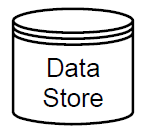
\includegraphics[width=0.9\columnwidth]{graphics/data-store}
	\caption{Data Store} 
	\label{fig:datastore} 
	\end{subfigure}
	\begin{subfigure}[b]{0.18\columnwidth}
		\centering
		
\includegraphics[width=0.8\columnwidth]{graphics/data-object}
		\subcaption{Data Object}
		\label{fig:dataobject}
	\end{subfigure}
	\caption{Data store and Data Objects according to the BPMN 2.0 standard \cite{bpmnstandard}} % Remove the [...] argument if the original caption should be used in the figure list.
	\label{fig:datastoreandobject} % \label has to be placed AFTER \caption (or \subcaption) to produce correct cross-references.
\end{figure}

\subsection{Bring the process model to an adequate granularity level}\label{granulartity}
The granularity of tasks modelled in an \gls{conceptual-bpmn} does differ from the granularity needed in an \gls{executable-bpmn}.
The goal of process automation is not to automate as much as possible but to have a centralized \gls{bpmn-wokflow-management-system} that does not only decide what task has to be done when but also who needs to be doing this task. \cite{freund2019real}
\\~\\Therefore consecutive tasks that are done by the same participant should be clustered together as one task to minimize handovers that have to be unnecessarily processed by the \gls{bpmn-wokflow-management-system}. \cite{fundamentals}
However there are some exception to this rule:
\begin{itemize}
	\item Tracking progress: In order to know how much the process has advanced it can be useful to split certain parts even if they are done by the same person. 
	\item Handling exceptions: If for a set of tasks that it performed by the same participant different erros and exceptions can occur, it might be useful to keep these tasks separated.
	\item Managing Resources: Sometimes consecutive tasks are performed by participants that have the same role, but could to be done by two different participants in order to use resources better. In this case it is also  to dis-aggregate the task accordingly.
 \end{itemize}

\subsection{Specify execution properties}
The final step in turning an \gls{conceptual-bpmn} executable is to specify the details of the implementation details of our \gls{bpmn} model. While the changes performed up to this step had an impact of the graphical representation, the execution properties are not graphically embedded into \gls{bpmn} but are encoded into the \gls{XML} representation of the BPMN-model. \cite{fundamentals} A schematic representation of the structure if \gls{bpmn} is provided in \ref{fig:bpmn-schema}. For the full specification of the BPMN-XML the \gls{xml}-schema can be found on the OMG-Website\cite{BPMN-xml-spec}. 
\begin{figure}[H]
		\centering
		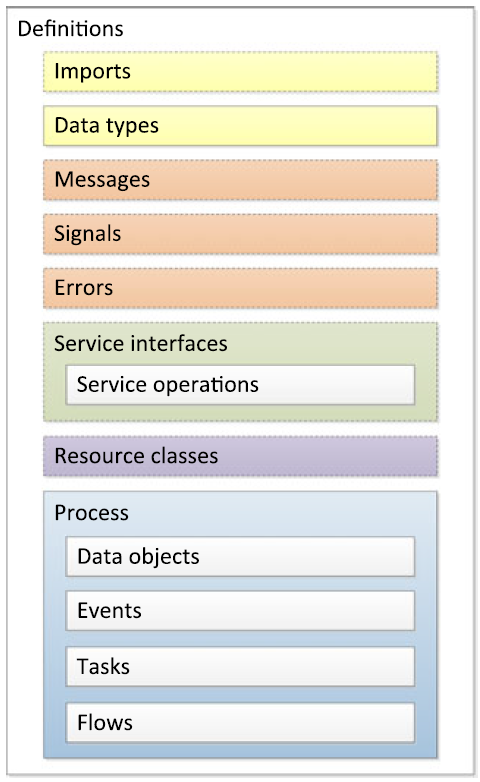
\includegraphics[width=0.3\columnwidth]{graphics/bpmn-schema}
		\caption{Structure of the BPMN format \cite{fundamentals}} 
		\label{fig:bpmn-schema} 
\end{figure}


\paragraph{Process Variables}~\\
In order to use data in different elements of our process, we need process variables that can be read, created and modified during the processes execution. Every Process variable has a \textbf{data type} that can either be simple (strings, integers, doubles, booleans, dates, times, ...) or complex (composed of other types). A complex Type needs to be described as an \gls{XSD}-Schema File.\\
\lstset{language=XML}
	\begin{lstlisting}[caption={The \gls{xml}-Schema Definiton for a complex type 'person'},captionpos=b]
<xs:element name="person">
	<xs:complexType>
		<xs:sequence>
			<xs:element name="name" type="xs:string"/>
			<xs:element name="address" type="xs:string"/>
			<xs:element name="city" type="xs:string"/>
			<xs:element name="country" type="xs:string"/>
		</xs:sequence>
	</xs:complexType>
</xs:element>
	\end{lstlisting}
\begin{lstlisting}[caption={An instance of the complex type 'person'},captionpos=b]
<person>
	<name>Dragana Sunaric</name>
	<address>Wiedner-Hauptstrasse 5</address>
	<city>1040 Wien</city>
	<country>Austria</country>
</person>
\end{lstlisting}


~\\The definition of common Errors, Messages and Escalations that are thrown or listened to by Events and Tasks are aslo part of the execution properties. Every Element has at least an \textbf{id} that identifies the given Element and a descriptive \textbf{name} of the element. \cite{bpmnstandard}
\paragraph{Messages}~\\
	\begin{lstlisting}
<message id="Message_ID" name="Message_NAME"/>
	\end{lstlisting}
\paragraph{Errors}~\\
Errors additionally have an \textbf{errorCode} that specifies the given Error. Events can listen for this specific error code and trigger when it is thrown.\\ 
	\begin{lstlisting}
<error id="Error_ID" name="Error_NAME" errorCode="Error_CODE"/>
	\end{lstlisting}
\paragraph{Escalations}~\\
Similar to errors, escalations additionally have an \textbf{escalationCode} that specifies the given Error and can be listened to by events. \\
	\begin{lstlisting}
<escalation id="Esc_ID" name="Esc_NAME" escalationCode="Esc_CODE"/>
\end{lstlisting}

\paragraph{Input and Output Variables}~\\
As mentioned earlier, Process Variables are active during the whole Process life-cycle. Apart from this data than can be accessed globally, it is also possible to define input and output values for each Task or Event in our process-model. These values are only visible within the Task or Event and have to be defined as an \gls{xsd}-Schema File (similarly to complex process variables). \cite{fundamentals}

\paragraph{Service Tasks}~\\
In order for service tasks to call external application or web-services, the interaction with the given service has to be defined in the process model. Connected services need to provide an service interface that describes the available service-operations and their parameters as well as return values. Service-operations can be synchronous, meaning the process instance waits for the operation to finish and to return a value or error code, or asynchronous, meaning the process does not wait for a response and carries on with the process after calling the service. Based on the service interface definition, input and output variables have to be defined for the service-call. The \gls{bpmn-wokflow-management-system} does this by copying the above mentioned Input values of the Task into the service call and if necessary, copy the output values of the service call into the output values of the Service task. \cite{fundamentals}

\subsection{Apply Naming Conventions}
\label{naming}
It is recommended to apply naming conventions for BPMN 2.0 diagrams. While there are many suggestions for naming conventions, none is defined by the BPMN 2.0 standard \cite{bpmnstandard}. The following is a suggestion for naming different BPMN elements based on  \cite{fundamentals}  \cite{suarez2010best} and \cite{radulian2020rethinking}. 

\paragraph{Events}~\\
Names of Events should start with a business object (noun) followed by a verb. In order to indicate that something just happened, the verb should be in the past participle form. The noun can be specified by an adjective in front. Examples for good Event names: 
\begin{itemize}
	\item Order delivered
	\item Large Order delivered
\end{itemize}

\paragraph{Tasks}~\\
Tasks should be named starting with a verb and followed by a business object (noun). The object can be specified using an adjective. If needed, the task name can also answer how the task will be accomplished by appending an explanation to the task name. Examples for good task names:
\begin{itemize}
	\item deliver order
	\item deliver large order
	\item deliver large order with truck 
\end{itemize}

\paragraph{Gateways}~\\
Gateways only need to be named if they are divergent exclusive Gateways. Divergent exclusive gateways should consist of at least a noun followed by a verb followed by a question mark to indicate what is evaluated at this gateway. Alternatively a whole questions can be asked. Examples for good gateway labels:
\begin{itemize}
	\item order delivered?
	\item was order delivered in time?
\end{itemize}

\paragraph{Sequence Flows}~\\
Sequence flows only need to be named if they come out if diverging Event based, exclusive or inclusive gateways. Sequence flows that follow one of those gateways should have labels that indicate the outcome of the gateways condition. 

\paragraph{General Rules}~\\
All Tasks, Events and Gateways should have a label. Sequence flows should have a label if they leave a exclusive, inclusive or event based gateway. Generally the naming convention should be in it consistent and for readability it is recommended to avoid long names. 

\chapter{Evaluating and Optimizing Executable Process Models}



\section{Six Sigma Approaches}
% Fundamentals and Handbook for process management
The first set of analysation and optimization techniques discussed in this chapter originate from the Six Sigma initiative. The name Six Sigma originates from the interval of $6\sigma$ in the normal distribution that indicates the aimed success rate of $99.99966\%$ \cite{siha2008business}\cite{vivekananthamoorthy2011lean} . A representation of the statistical meaning can be see in figure \ref{fig:six-sigma}. Apart from the goal to decrease the error rate, $6\sigma$ is also an methodology for systematically improving process quality \cite{tennant2017six}.

\begin{figure}[H]
		\centering
		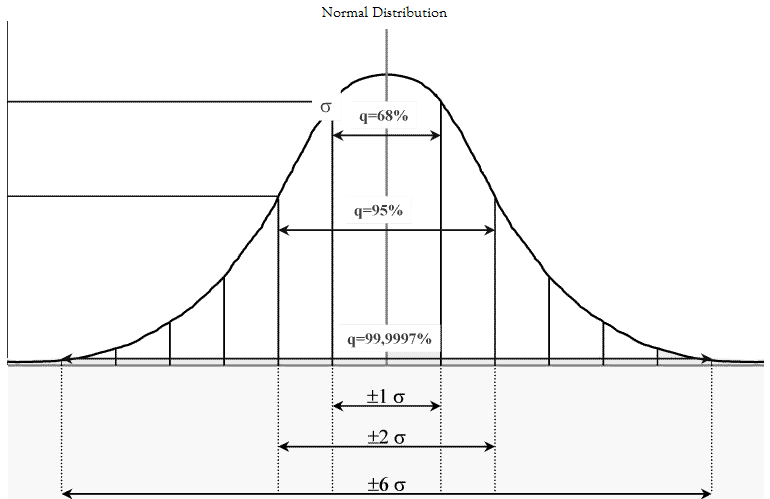
\includegraphics[width=0.7\columnwidth]{graphics/six-sigma}
		\caption{The standard normal distribution showing the $6\sigma$ interval (graphic from \cite{vivekananthamoorthy2011lean})} 
		\label{fig:six-sigma} 
\end{figure}

Applied in the context of (executable) business processes, Six Sigma provides a set of methods to identify and eliminate inefficient or needless steps in a process \cite{vom2014handbook}. While countless tools are available as part of Six Sigma, the two main methodologies applied in these tools are \gls{DMAIC}, used for improving existing processes, and \gls{DMADV}, used when creating new processes \cite{selvi2014six} .


In the following, a few selected Six Sigma methods are described that apply the \textbf{DMAIC} and  \textbf{DMADV} approach, these being:  
\begin{itemize}
	\item SIPOC Analysis
	\item Check Sheets
	\item Cause and Effect Diagram
	\item Root Cause Analysis
	\item Quality Function Deployment (QFD)
\end{itemize}

To demonstrate a few of the following methodologies, the exemplary \textit{Missing Part Process} will be used. The fictional process demonstrates what happens when a customer of a furniture shop reports a missing part in his/her order and requests a new part to be shipped. The corresponding \gls{bpmn}-model is shown in Figure \ref{fig:missing-part-process}

\begin{figure}[H]
	\centering
	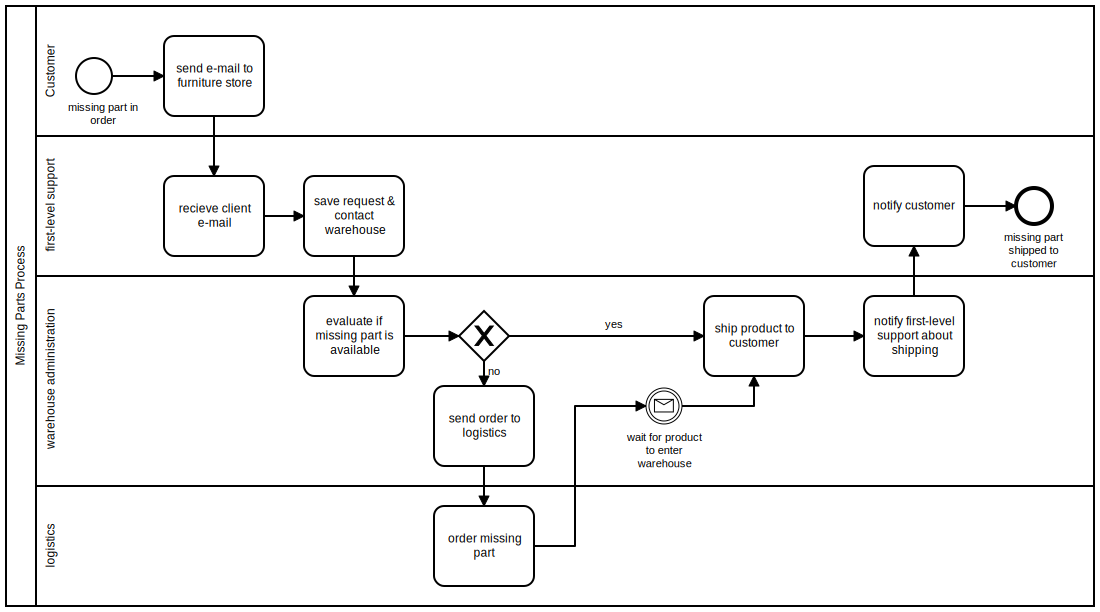
\includegraphics[width=1\columnwidth]{processes/missing-parts-process/missing-parts-process}
	\caption{The \gls{bpmn} model for the \textit{Missing Part Process}} 
	\label{fig:missing-part-process} 
\end{figure}

\subsection{SIPOC Analysis}
The SIPOC analysis is a tool used in the \textbf{Define} phase of \gls{DMAIC} and \gls{DMADV} and should provide more detailed information about each process step than the \gls{bpmn} model  \cite{vom2014handbook}. 

The outcome of a SIPOC analysis is a table, containing the following information for each task in the process \cite{toutenburg2008six}: 
\begin{itemize}
	\item \textbf{S}upplier: provides the input for this task and influence the output the supplier can be internal or external. 
	\item \textbf{I}nput: Resources, data or material needed for this task provided by the suppliers. 
	\item \textbf{P}rocess: the series of actions taken in this task. This can also be a subprocess. 
	\item \textbf{O}utput: represent the result of this process task and provide value for the customer
	\item \textbf{C}ustomer: the customer that benefits from the output of this task (can be external or internal of the organization)
\end{itemize}

When this method is applied to the \textbf{Missing Part Process} the resulting SIPOC table looks like this: 
%TODO Process


\subsection{Check Sheets}

\subsection{Pareto Analysis}

\subsection{Cause and Effect Diagram}

\subsection{Root Cause Analysis}

\subsection{Quality Function Deployment (QFD)}

\section{Other Qualitative Measures}

\subsection{Value Added Analysis (VAA)}


\section{Quantitative Analysis}
The issue with qualitative methods for process improvement is the inability to quantify the impact of theyr application. In order to measure and justify changes in the status quo process we need quantitative methods for analyzing processes. In the context of \gls{bpm}, assessable measures about three different dimensions of a process can be investigated : The process as a whole, resources involved in the process and individual Tasks in a process. \cite{fundamentals}

Before discussing methods for measuring process performance, it is necessary to define what is measured. The four key performance measures examined in this chapter are: cost, time, quality and flexibility. \cite{fundamentals}

The following chapter will present methods for qualitative analysis of processes. Starting with the definition of the four dimensions of process performance: cost, time, quality and flexibility. Afterwards the following methods for measuring performance will be described: 

\begin{itemize}
	\item Flow Analysis
	\item Queues
	\item Simulation
\end{itemize}
\subsection{Performance Measures}
As mentioned above, the performance of a process can be measured using the four dimensions:  cost, time, quality and flexibility. 
\paragraph{Cost}~\\

\paragraph{Time}~\\
\textit{Cycle time} or \textit{throughput time} is the time it takes for a process from start to finish \cite{Six-sigma-terms}. In the case of the \textit{Missing Part Process} shown in \ref{fig:missing-part-process}, the cycle time would be the time that elapses from the moment the customer notices that a part is missing to the time the missing Part is shipped. While the \textit{Cycle time} of the whole process as a metric is highly relevant for client satisfaction, it is on its own usually not tangible when it comes to improvement of the process. The \textit{cycle time} usually consists of two constituents \cite{fundamentals}:
\begin{itemize}
	\item \textit{Processing time}: The time where the request is actively processed, meaning the process participants (e.g. people or software) actually spend this time handling the process. 
	\item \textit{Waiting time}: The time a process spends waiting. Waiting time includes the time the process is waiting in a queue for resources to finish the processing of previous processes and other waiting times, like waiting for the product to enter the warehouse in the \textit{Missing Part Process}
\end{itemize}
\paragraph{Quality}~\\

\paragraph{Flexibility}~\\

\subsection{Flow Analysis}
The Idea behind (work)flow analysis is to estimate the overall performance of a process given the performance of individual tasks.  

Flow analysis is especially useful in order to analyze alternative process designs. By considering the performance of each step in the process, the benefit of process redesigns can be quantified and the impact of automating individual tasks becomes visible.

In the following the analyzed performance measure that is looked at will be execution time. 
\paragraph{Sequential Tasks}~\\
The first calculation starts with sequential tasks or blocks. The execution time of consecutive tasks in a process can be added together to calculate the total time of those two tasks. 
Considering the tasks in \ref{fig:sequential-tasks} where the runtime of each task is brackets below the task name, this would result in a process time of 30s for this block. \cite{ha2006approximate} \cite{fundamentals}

\begin{figure}[H]
	\centering
	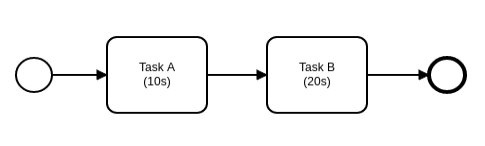
\includegraphics[width=0.5\columnwidth]{graphics/sequential-tasks}
	\caption{a process with two sequential executed tasks} 
	\label{fig:sequential-tasks} 
\end{figure}

Considering a more general process model $P$ with sequential blocks $B_1,B_2 ... B_n$ the runtime $R_P$ of process $P$ ca be calculated using the formula \ref{eq:sum-seq}. 
\begin{equation}\label{eq:sum-seq}
	R_P = \displaystyle\sum_{i=1}^{n} B_i
\end{equation}

\paragraph{Parallel Tasks}~\\
The cycle time of parallel tasks or blocks can be calculated using the maximum time of the two parallel blocks. Given the parallel block in \ref{fig:parallel-tasks}, this would result in a process time of 20s for this block.\cite{fundamentals}
\begin{figure}[H]
	\centering
	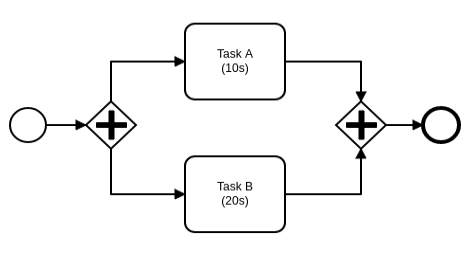
\includegraphics[width=0.5\columnwidth]{graphics/paralell-tasks}
	\caption{a process with two parallel executed tasks} 
	\label{fig:parallel-tasks} 
\end{figure}

Considering a more general process model $P$ with parallel blocks $B_1,B_2 ... B_n$ the runtime $R_P$ of process $P$ ca be calculated using the formula \ref{eq:sum-par}. 
\begin{equation}\label{eq:sum-par}
	R_P = \operatorname*{arg\,max}_i B_i
\end{equation}

\paragraph{Alternative Sequence Flows}~\\
When having two or more alternative sequence flows with different execution times, additional knowledge about the likelihood of those alternatives is needed \cite{fundamentals}. When looked at the alternative executed tasks in \ref{fig:alternative-tasks}, the average cycle time can be estimated by multiplying the probability of the two alternatives with the execution time of the tasks and summing up the results. This results in $10 * 70\% + 20 * 30\% = 13s$ estimated execution time. 

\begin{figure}[H]
	\centering
	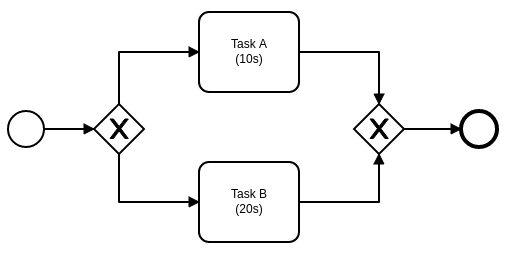
\includegraphics[width=0.5\columnwidth]{graphics/alternative-tasks}
	\caption{a process with two alternative sequence flows} 
	\label{fig:alternative-tasks} 
\end{figure}

Generally, the cycle time $R_P$ of a process $P$ with one or more alternative blocks, that have the runtimes $B_1,B_2 ... B_n$ and a likelihood of $p_1,p_2 ... p_n$ respectively, is estimated with the formula \ref{eq:alternative-seq}. \cite{fundamentals}

\begin{equation}\label{eq:alternative-seq}
	R_P = \displaystyle\sum_{i=1}^{n} B_i * p_i
\end{equation}

\paragraph{Repeating Tasks}~\\
According to the BPMN-Standard\cite{bpmnstandard} defined by OMG, there are multiple ways to indicate that a task or sequence is executed more than once: 

\begin{itemize}
	\item \textbf{Activity Looping}: A loop in the bottom center of the activity indicates, that this task si performed more than once. The definition on when this task repeats is specified in the \textit{loopCharacteristics}-XML Element.
	\begin{figure}[H]
		\centering
		\includegraphics[width=0.5\columnwidth]{graphics/activity-looping}
		\caption{A Task with Activity Looping} 
		\label{fig:activity-looping} 
	\end{figure}
	\item \textbf{Sequence Flow Looping}: Whenever a whole sequence flow instead of a task needs to be repeated, a \textit{Sequence Flow Looping}-pattern can be used where the looping condition is defined within a exclusive gateway. The default flow points back to the start of the repeating sequence flow. 
	\begin{figure}[H]
		\centering
		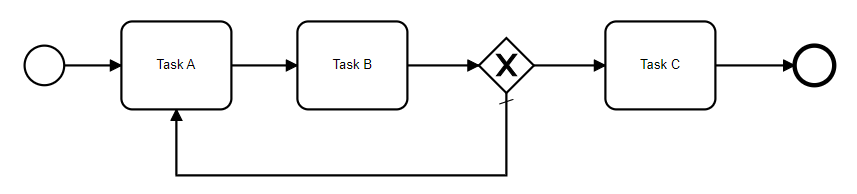
\includegraphics[width=0.5\columnwidth]{graphics/sequence-flow-looping}
		\caption{The Sequence Flow Looping Pattern} 
		\label{fig:sequence-flow-looping} 
	\end{figure}
	\item \textbf{Multiple Instances}: Three lines in the bottom of the task indicate that a task is executed multiple times - once for every instance or element. There are two kinds of muli-instance tasks, sequential, meaning the instances are processes one after another and parallel, meaning the instances are processed at the same time. 
	\begin{figure}[H]
		\centering
		\includegraphics[width=0.5\columnwidth]{graphics/muliti-instance-tasks}
		\caption{Mulitple Instance Tasks} 
		\label{fig:muliti-instance-tasks} 
	\end{figure}
\end{itemize}


% Cycle time using flow analysis
%	additive when sequential
%	Gates:
%		OR: percentage of when option ab and B is used
%		paralell: maximum of the two options
%		inclusive: more complicated....
%	
% 	Cycle time efficnecy : how much time is being waited / can we reduce it
%	Littles Law
%	empirical vs. estimated data



\subsection{Queues}
%see https://link.springer.com/content/pdf/10.1007/11837862.pdf:
%An Approximate Analysis of Expected Cycle Time in Business Process Execution
As mentioned before, the \gls{cycle-time} of a process consists of the time the process is actively executed (\textit{processing time}) and the time the process spends waiting (\textit{waiting time}). In the previous section basic flow analysis was introduced to approximate and analyze these measures.  
While the processing time can be approximated using basic flow analysis, getting an idea about the total expected waiting time of a process is more complex, since flow analysis as it is has no tool to estimate queuing time. 

In order to bridge this gap, the flow analysis can be extended using an queuing approximation algorithm as it is described in this paper\cite{ha2006approximate}.

% TOOD describe flow analysis with queuing analysis

\subsection{Simulation}


\subsection{Cycle Time Efficiency}
\subsection{Littles Law}
\section{Benchmarking Processes}


%H. Harrington - Business Process Improvement chapter 9 

\chapter{Concept and Implementation}
The following chapter will describe the software that was implemented as part of this thesis. The software is supposed to read in an \gls{bpmn}2.0 Diagram and return a set of suggestions how this BPMN can be improved according to the best-practices described in the first chapters.

This chapter will start with describing the technical implementation and used technologies that were used as well as details on how the software is structured and how it can be used. 
Moreover, this chapter will describe the REST-interface that was implemented and Objects returned by the software. 

Finally the suggestions that can be made to an executable BPMN will be described in section \ref{last}. Some of this suggestions will not be suitable to automation. Explanations on why certain suggestions where implemented and others not will also be provided in this section.
\section{Software Architecture}
The Software was implemented as an Spring Boot Server\cite{spring-boot} Application. The software was developed using git\cite{git} as version control system and the git project is available as an open source project on \url{https://github.com/dsunaric/epms-service}.\\~\\

This software is implemented using maven\cite{maven} as a build-tool, therefore software artifacts can be added to the local repository using the command \verb|mvn install|. This also generates the API sources into the \verb|target| directory. After that the packaged .jar file can be run using the command \verb|java -jar target/*.jar|. 


\subsection{BPMN Processing}
For reading in and processing the BPMN models the Camunda-Model-API\cite{camunda-model-api} was used. The reason for that was the detailed documentation and better usability compared to using an XML parser. The Camunda Model API is able to process most BPMN 2.0 elements. A list of supported elements can be found in the \textit{instance} package\cite{camunda-model-api-spoorted-elements}.
% BPMN 2.0
% cmaunda BPMN model API
\subsection{Folder structure}~\\
The following visualizes and describes the important parts of the projects folder structure:
\dirtree{%
	.1 epms-service.
	.2 src.
		.3 main.
			.4 java.
				.5 at.
					.6 epms.
						.7 api\DTcomment{contains implemented API}.
						.7 entity.
						.7 mapper.
						.7 service\DTcomment{contains suggestion logic}.
							.8 validator\DTcomment{contains validators for the specified best-practices}.
			.4 resources.
				.5 api\DTcomment{contains API specification}.
				.5 config\DTcomment{contains Spring Boot configuration}.
			.4 webapp\DTcomment{contains generated sources for potential clients}.
	.2 target\DTcomment{contains executable .jar file after build} .
}

\section{Interface}
The API was designed and developed using OpenAPI and Swagger\cite{swagger}. The OpenAPI definition is written in one \textit{.yaml} file which is located in the folder\\ \verb|epms-service/src/main/resources/api|.

After Starting the Software, the API description is accessible on \\ \verb|localhost:8080/documentation/v3/api-docs| and can directly be used for code generation by potential frontend applications. 

The application has only one REST-Endpoint, \verb|GET /suggestions|. This endpoint has the process model as request body and returns a list of \textbf{AppliedRules} Objects. 

One \textbf{AppliedRule} object has the following attributes:
\begin{itemize}
	\item \textbf{title}: The title of the applied Rule
	\item \textbf{description}: The description of the rule. Explains when the Rule applies.
	\item \textbf{details}: Explains details about the rule and gives explanation about the effected elements.
	\item \textbf{effectedElements}: A list of elements that violate this rule. The id, name and type (event or task) of the effected element is returned.
\end{itemize} 
\section{Suggestions for improvement}\label{last}
This section describes a set of possible suggestions for improving a BPMN Model. Not all of those rules where implemented as some are not suitable for automation or would be beyond the scope of this thesis. 

\subsection{Comply with Naming Conventions}\label{naming-con}
BPMN models, no matter if conceptual or executable, should meet naming conventions as it is described in section \ref{naming}. One aspect of naming conventions is the recommended maximum length of five words for any label. 

Since natural language processing would go beyond the scope of this thesis and naming conventions apply to not only executable BPMN, this suggestion for improvement was not fully automated in the context of this thesis. Because of its simplicity, suggesting to rename a element when the label is too long (greater than five words) was implemented.

\subsection{Extend automation boundaries}
The first step of turning an conceptual process model executable is identifying the automation boundaries \ref{automation}. In order to optimize na existing process one could think of extending those existing boundaries and brainstorming ideas to automatize tasks that are not yet automatable. 

This requires a lot of domain specific knowledge and can therefore not be simply implemented.

\subsection{Eliminate Manual Tasks}\ref{soft-manual}
As describes in section \ref{manual} Manual Tasks should not be part of an executable BPMN diagram and should if possible be automated using service tasks or, if that is not possible, be replaced by user tasks. 

Manual tasks are identified by the software. The returned effected elements represent a list of manual tasks in the given diagram.

\subsection{Complete the process model}
Another manual step to improve a process model, is making sure the process model is complete section \ref{complete}.

Since this would also require domain specific knowledge, the software does not include analyzing the process model for incompleteness.

\subsection{No two consecutive Tasks handled by the same resource}\label{merge-section}
Two task that are executed one after the other should be merged, if they have the same enitity executing the task. As described in section \ref{granulartity}, bringing the model to an adequate granularity level minimizes handovers and overhead. In case of User tasks this means the same usergroup is executing both tasks. Automated Tasks that follow each other should also always be merged to minimize flownodes.


The software recognizes such consective tasks return a list of effected elements that represent the tasks that can be merged with its direct successor. In case that three or more tasks can be merged, this algorithm will return every task that can be merged with its successor on its own. Therefore if ``task1`` , ``task2`` and ``task3`` can be merged all together, the algorithm will return ``task2`` and ``task3`` as effected elements.

An example on when this rule is satisfied can be found in figure \ref{fig:example-EX}. The software will return \textit{Task A}, \text{Task B} and \textit{Task D} as effected elements, indicating, that  \textit{Task D} should be merged with its successor ( \textit{Task E}),  \textit{Task A} should be merged with  \textit{Task C} and  \textit{Task B} should be merged with  \textit{Task C}, therefore merging all three Tasks ( \textit{Task A}, \textit{Task B} and  \textit{Task C})together. An example for an resulting process model, after this suggestions are applied, can be found in figure \ref{fig:example-EX-fix}.

\begin{figure}[H]
	\centering
	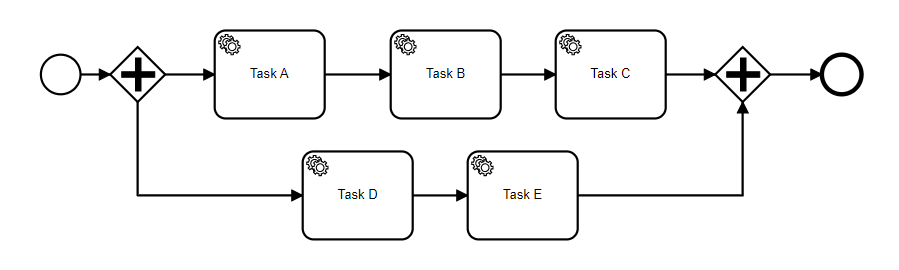
\includegraphics[width=0.9\columnwidth]{graphics/merge-suggestion-1}
	\caption{Example of a process where tasks can be merged together} 
	\label{fig:example-EX} 
\end{figure}

\begin{figure}[H]
	\centering
	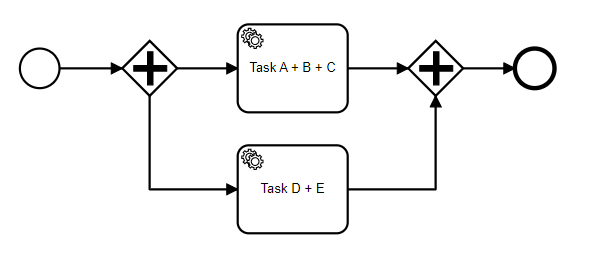
\includegraphics[width=0.7\columnwidth]{graphics/merge-suggestion-2}
	\caption{change necessary for the process in \ref{fig:example-EX} so satisfy this rule} 
	\label{fig:example-EX-fix} 
\end{figure}

\subsection{Inclusive Gateways over combining parallel and exclusive Gateways}\ref{inc-sw}
In order to save flownodes, inclusive gateways should be used instead of a parallel gateway followed by one or more exclusive gateways. An example for this kind of pattern is shown in \ref{fig:example-GW}.

\begin{figure}[H]
	\centering
	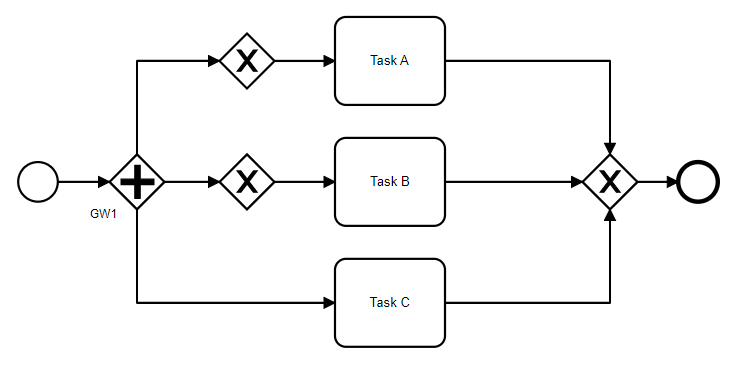
\includegraphics[width=0.9\columnwidth]{graphics/exclusive-suggestion-1}
	\caption{Example for a parallel gateway followed by one or more exclusive gateways} 
	\label{fig:example-GW} 
\end{figure}

The software applies this rule whenever a parallel gateways is followed by one or more exclusive gateways. The returned effected elements are a list of parallel gateways that are followed by one or more exclusive gateways in the given diagram. In the example shown in  \ref{fig:example-GW}, the returned element would be \textit{GW1} and the change to comply with this rule would be shown in \ref{fig:example-GW-fix}
\begin{figure}[H]
	\centering
	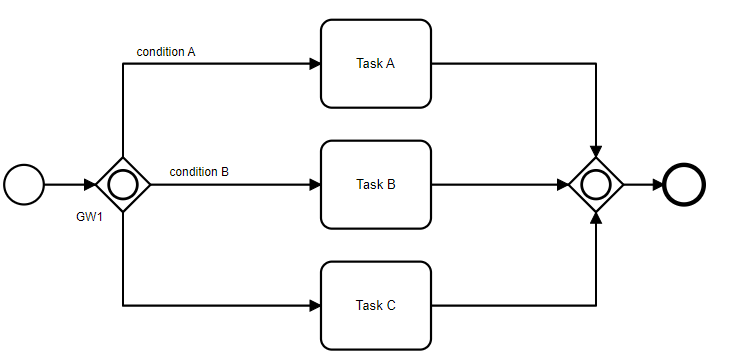
\includegraphics[width=0.9\columnwidth]{graphics/exclusive-suggestion-2}
	\caption{change necessary for the process in \ref{fig:example-GW} so satisfy this rule} 
	\label{fig:example-GW-fix} 
\end{figure}

\subsection{Value Added Analysis}
In order to eliminate tasks in a process that have limited value for the customer, a value added analysis as explained in section \ref{vaa} can be performed.  

This would also require domain specific knowledge and is therefore not done by the software. 

\subsection{Evaluate Suggestions Quantitative}

Finally, all process models as a result of applying any of those suggestions made by the software or manually, can be evaluated against each other using quantitative measures. The section \ref{quant} describes approaches to estimating quantitative measures using flow analysis. 

Since BPMN 2.0 has no option to integrate estimations for quantitative measures for processes or tasks, and estimation would require detailed knowledge about the process at hand, this will not be implemented.

\chapter{Case Study}
\section{Apply naming conventions}
%see  https://docs.camunda.io/docs/components/best-practices/modeling/creating-readable-process-models/
%   & https://docs.camunda.io/docs/components/best-practices/modeling/naming-bpmn-elements/
\subsection{renaming tasks}
\subsection{renaming gateways}
\subsection{rename events}

\section{Review Manual Tasks}
\section{Bring the model to an adequate granularity level}
\section{Eliminate Antipatterns}
\subsection{Event based gateway vs paralell + exclusive}

\section{Validation of execution properties}



\chapter{Conclusion}
\todo{write conclusion}

\backmatter

% Use an optional list of figures.
\listoffigures % Starred version, i.e., \listoffigures*, removes the toc entry.

% Use an optional list of tables.
\cleardoublepage % Start list of tables on the next empty right hand page.
\listoftables % Starred version, i.e., \listoftables*, removes the toc entry.

% Use an optional list of alogrithms.
\lstlistoflistings
\addcontentsline{toc}{chapter}{List of Algorithms}

% Add an index.
\printindex

% Add a glossary.
\printglossaries

% Add a bibliography.
\bibliographystyle{plain}
\bibliography{intro}

\end{document}